%!TEX root = ../dissertation.tex

\chapter{Сокращение пространства поиска при генерации детерминированных конечных автоматов с использованием сведения к задаче выполнимости}
\label{sec:space}

Настоящая глава посвящена разработке предикатов нарушения симметрии, основанных на алгоритмах обхода графа в ширину и в глубину, для сокращения пространства поиска при решении задачи выполнимости, а также разработке, реализации и экспериментальным исследованиям методов генерации ДКА по заданным примерам поведения, использующих данные предикаты.

%------------------------------------------------------------------------------------------------------

\section{Предикаты нарушения симметрии на основе алгоритма обхода графа в глубину}
\label{sec:space:dfs}

В настоящем разделе описывается разработка предикатов нарушения симметрии на основе алгоритма обхода графа в глубину.

Предикаты нарушения симметрии, основанные на алгоритме обхода графа в ширину, описанные в разделе~\ref{sec:review:sym-breaking:bfs-based}, помогли существенно улучшить производительность существующих точных методов генерации ДКА по заданным примерам поведения.
Логичным продолжением данного исследования является разработка предикатов нарушения симметрии на основе алгоритма обхода графа в глубину (depth-first search~--- DFS).
Пример DFS пронумерованного автомата представлен на рисунке~\ref{img:dfs-ex}.
На рисунке~\ref{img:dfs-tree-ex} представлено соответствующее ему DFS дерево.

\begin{figure}[ht]
  \centering
  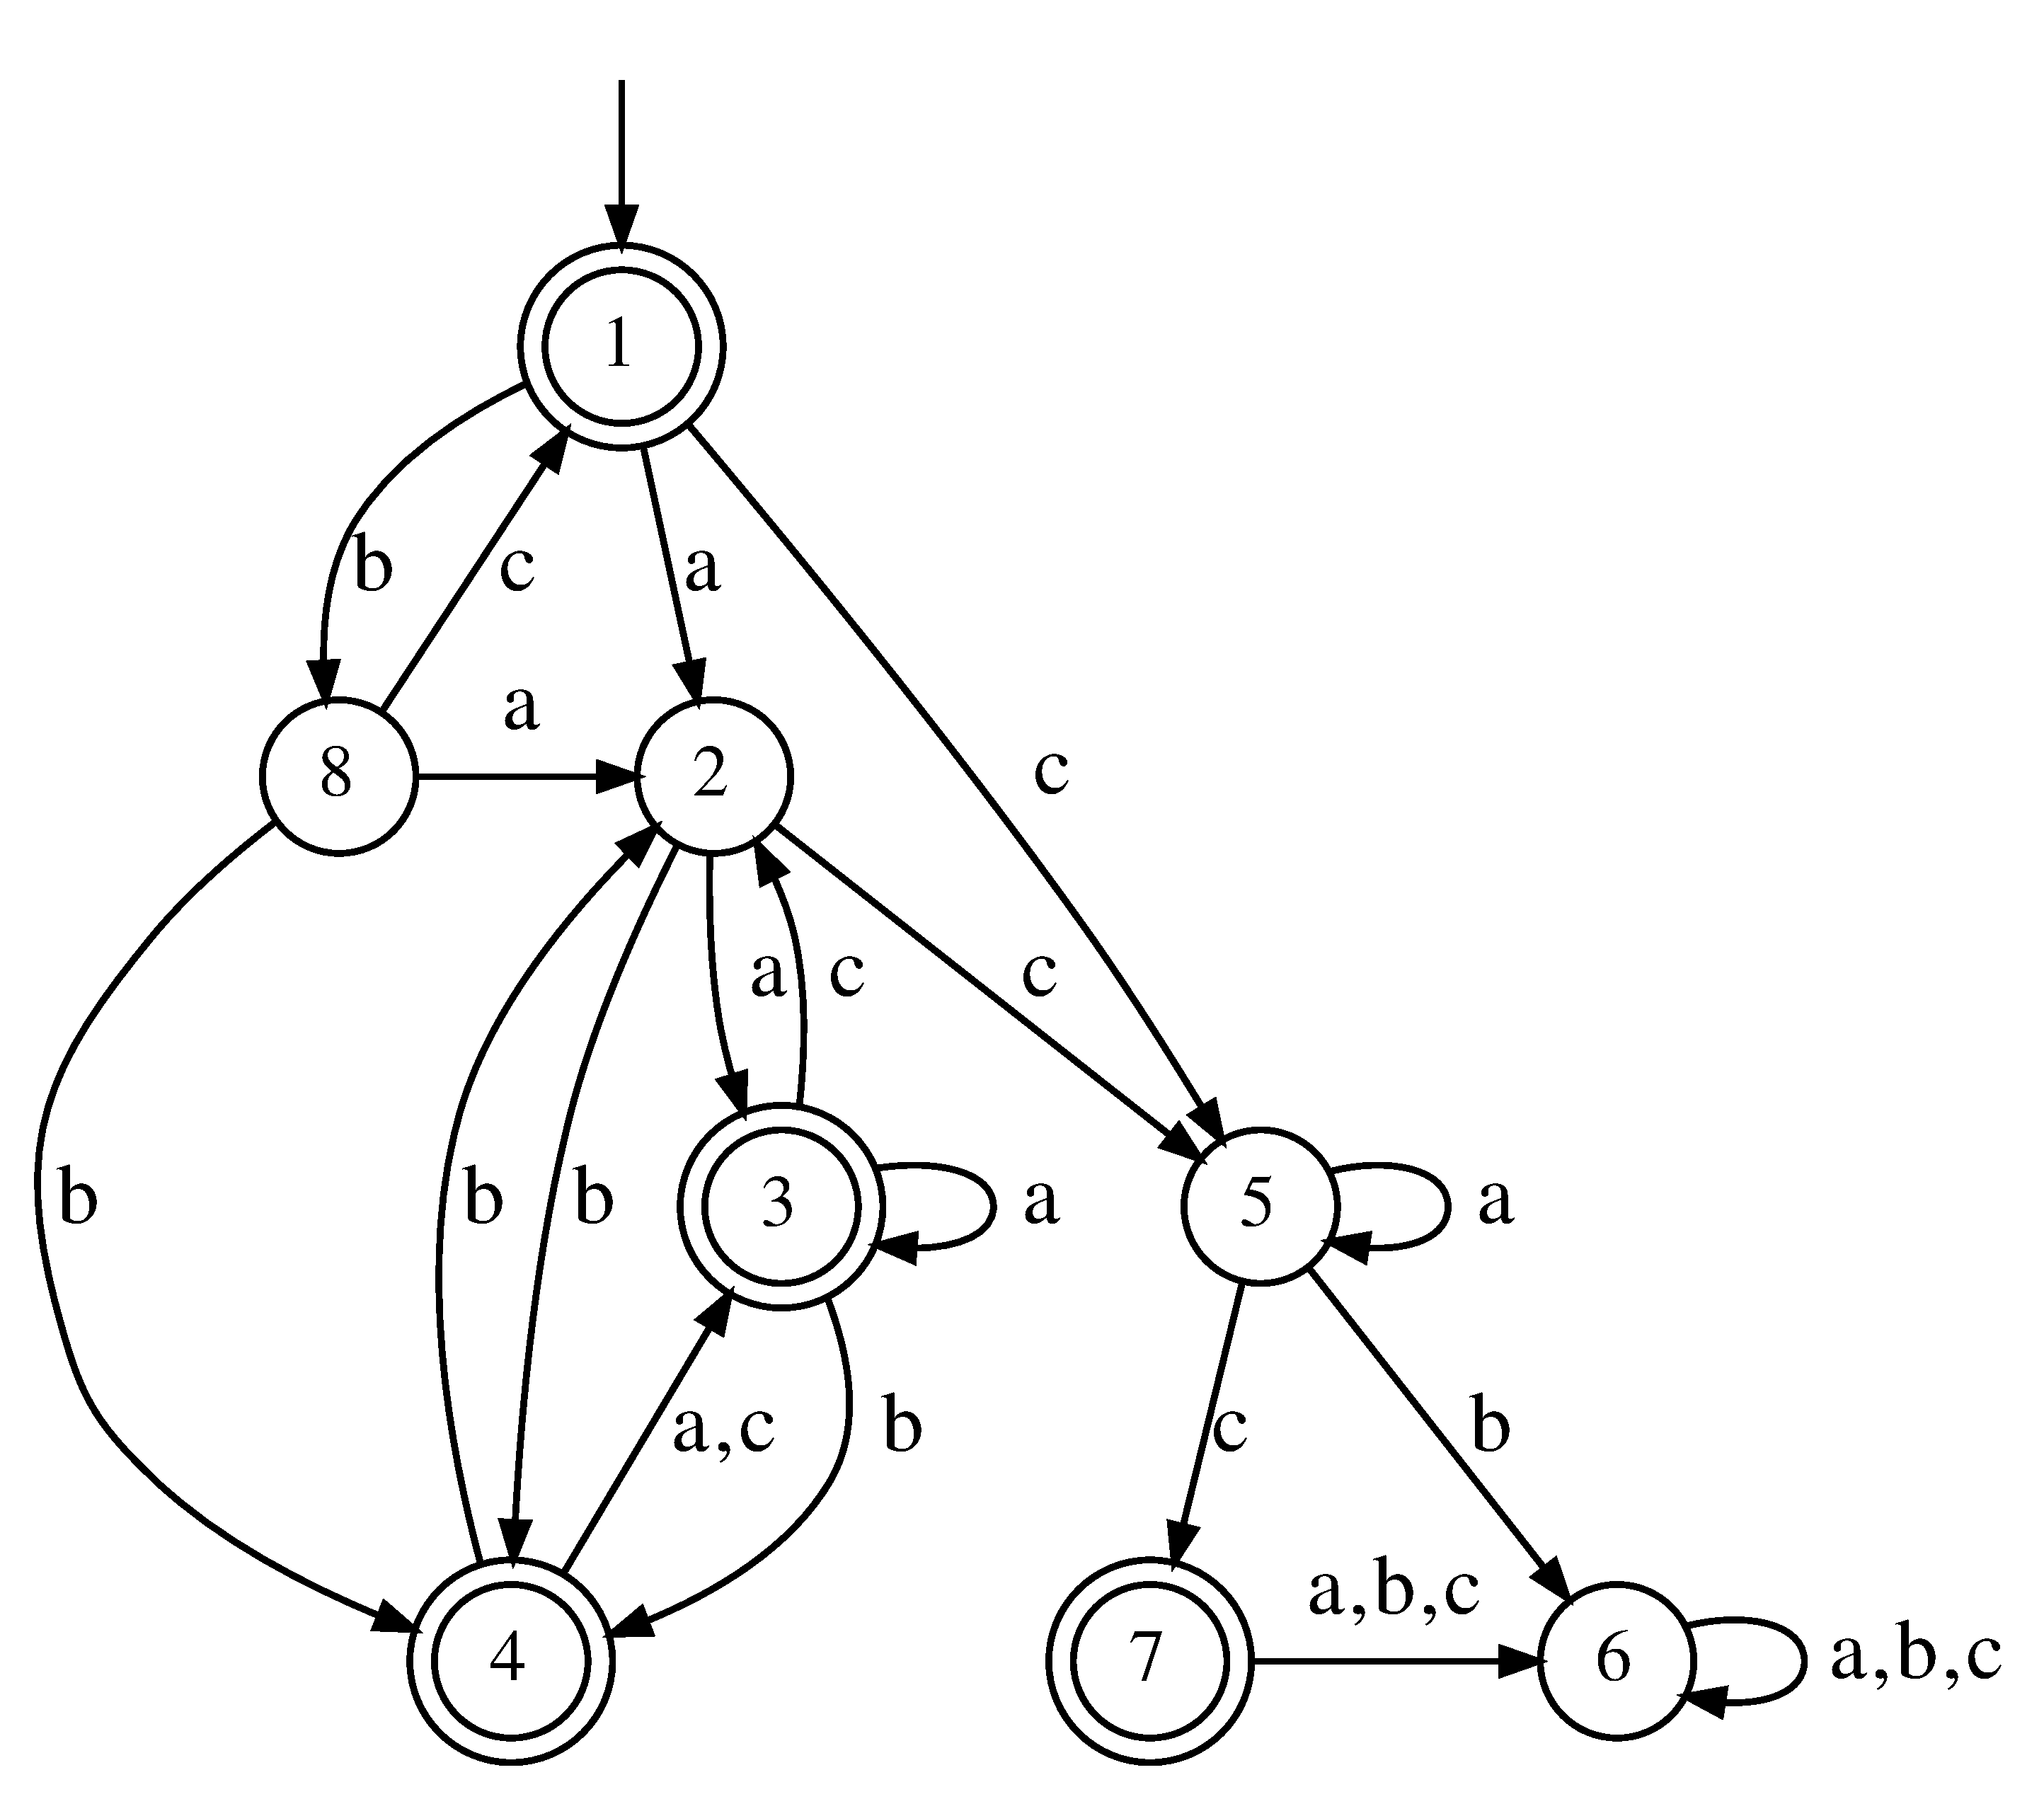
\includegraphics[scale=0.12]{img/datamod/DFS-example.eps}
  \caption{Пример DFS пронумерованного автомата}
  \label{img:dfs-ex}
\end{figure}

\begin{figure}[ht]
  \centering
  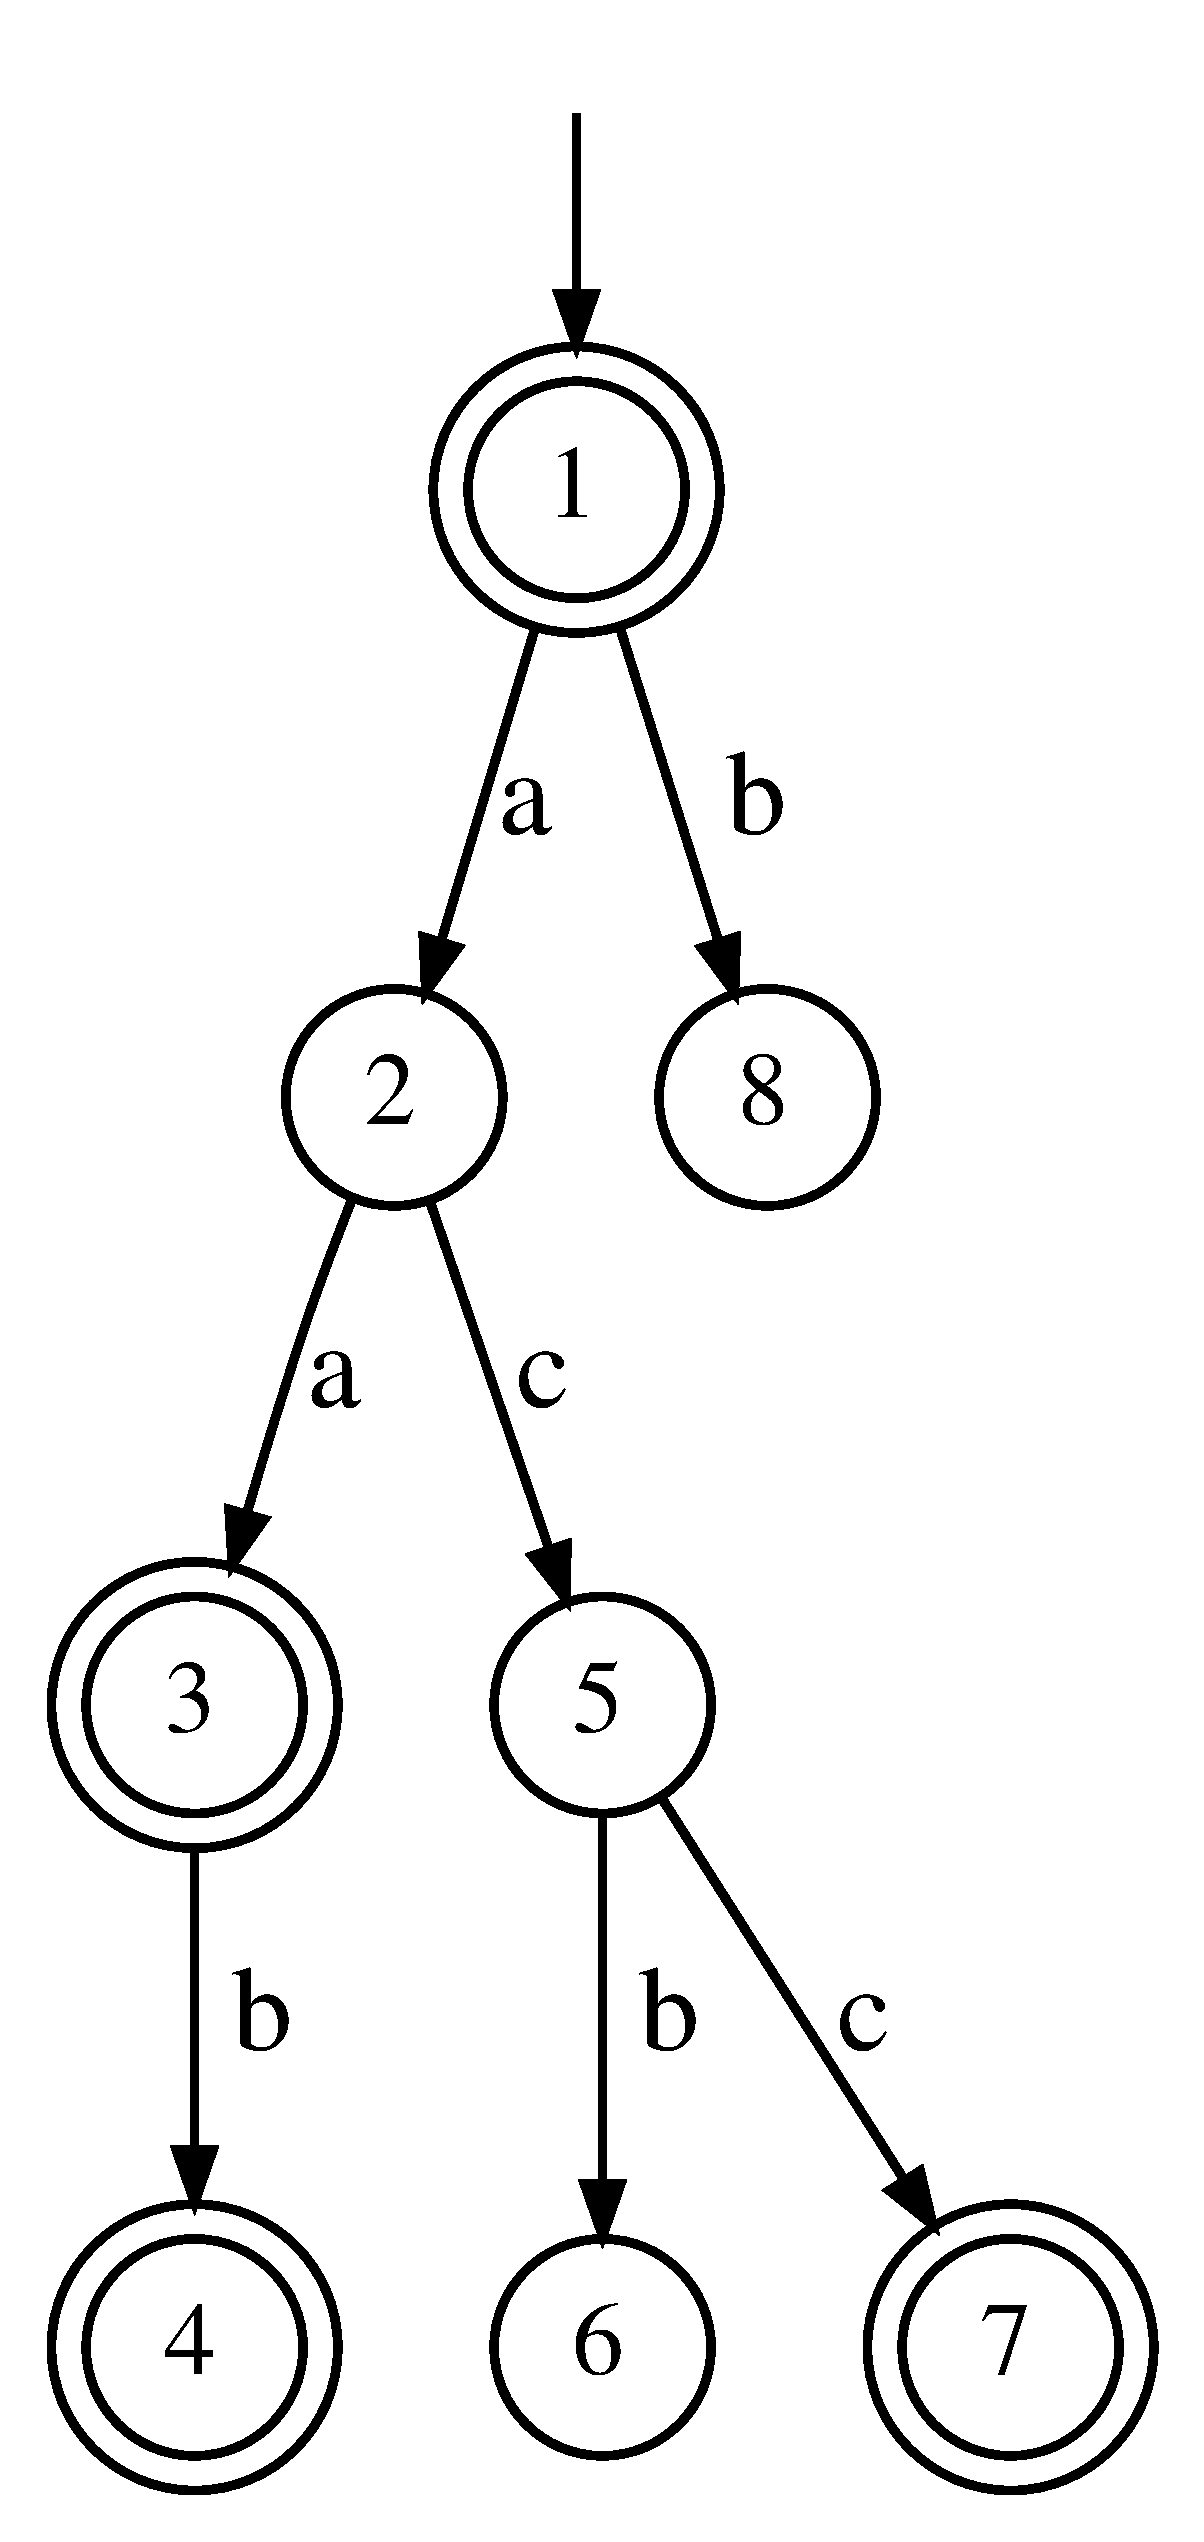
\includegraphics[scale=0.12]{img/datamod/DFS-tree.eps}
  \caption{Дерево DFS для автомата, представленного на рисунке~\ref{img:dfs-ex}}
  \label{img:dfs-tree-ex}
\end{figure}

%------------------------------------------------------------------------------------------------------

\section{Компактные предикаты нарушения симметрии на основе алгоритма обхода графа в ширину} 
\label{sec:space:tight}

Кодирование свойства BFS пронумерованности автомата, описанное в разделе~\ref{sec:review:sym-breaking:bfs-based}, состоящее из $\mathcal{O}\left(M^{3} + M^{2} \times L^{2}\right)$ дизъюнктов, слабо применимо на практике для ДКА большого размера, то есть при большом $M$. 
В настоящем разделе описывается как модифицировать предикаты нарушения симметрии, рассмотренные ранее, таким образом, что для их булевого кодирования понадобится только $\mathcal{O}\left(M^{2} \times L\right)$ дизъюнктов.

\inote{подумать о подразделах}

%----------------------------------------------------------------------------------------

\subsection{Ревизия существующего кодирования}
\label{sec:space:tight:review}

В данном подразделе повторно кратко приводятся наборы дизъюнктов, с помощью которых кодируются предикатов нарушения симметрии на основе алгоритма BFS, приведенные в разделе~\ref{sec:review:sym-breaking:bfs-based}.

\begin{equation}
\label{eq:t-def}
  \bigwedge_{1 \leq i < j \leq M} \left(t_{i,j} \leftrightarrow y_{i,l_{1},j} \vee y_{i,l_{2},j} \vee \ldots \vee y_{i,l_{L},j} \right)
\end{equation}
%
\begin{equation}
\label{eq:p-def}
  \bigwedge_{1 \leq i < j \leq M} \left(p_{j,i} \leftrightarrow t_{i,j} \wedge \neg t_{i - 1,j} \wedge \neg t_{i - 2, j} \wedge \ldots \wedge \neg t_{1,j}\right)
\end{equation}
%
\begin{equation}
\label{eq:p-alo}
  \bigwedge_{2 \leq j \leq M} \left(p_{j,1} \vee p_{j,2} \vee \ldots \vee p_{j,j - 1}\right)
\end{equation}
%
\begin{equation}
\label{eq:p-order}
  \bigwedge_{1 \leq k < i < j \leq M} \left(p_{j,i} \rightarrow \neg p_{j + 1, k}\right)
\end{equation}
%
\begin{equation}
\label{eq:m-def}
  \bigwedge_{1 \leq i < j \leq M} \bigwedge_{1 \leq n \leq L} \left(m_{i,l_{n},j} \leftrightarrow y_{i,l_{n},j} \wedge \neg y_{i,l_{n - 1}, j} \wedge \neg y_{i,l_{n - 2}, j} \wedge \ldots \wedge \neg y_{i,l_{1},j} \right)
\end{equation}
%
\begin{equation}
\label{eq:m-order}
  \bigwedge_{1 \leq i < j \leq M} \bigwedge_{1 \leq k < n \leq L} \left(p_{j,i} \wedge p_{j + 1, i} \wedge m_{i,l_{n}, j} \rightarrow \neg m_{i, l_{k}, j + 1}\right)
\end{equation}

Изучив формулы, приведенные выше, можно заключить, что:
\begin{enumerate}
  \item формула~\eqref{eq:t-def} содержит $\mathcal{O}\left(M^{2} \times L\right)$ дизъюнктов;
  \item формула~\eqref{eq:p-def} содержит $\mathcal{O}\left(M^{3}\right)$ дизъюнктов;
  \item формула~\eqref{eq:p-alo} содержит $\mathcal{O}\left(M\right)$ дизъюнктов;
  \item формула~\eqref{eq:p-order} содержит $\mathcal{O}\left(M^{3}\right)$ дизъюнктов;
  \item формула~\eqref{eq:m-def} содержит $\mathcal{O}\left(M^{2} \times L^{2}\right)$ дизъюнктов;
  \item формула~\eqref{eq:m-order} содержит $\mathcal{O}\left(M^{2} \times L^{2}\right)$ дизъюнктов.
\end{enumerate}
%
Таким образом, будет предложено новое кодирование для свойств, ранее выраженных формулами~\eqref{eq:p-def}, \eqref{eq:p-alo}, \eqref{eq:m-def} и \eqref{eq:m-order}.

Прежде всего, заметим, что формула~\eqref{eq:p-alo} задает свойство, что у каждого состояния $d_{j}$ (кроме начального) автомата $\mathcal{D}$ существует как минимум один родитель в дереве BFS, при этом с меньшим номером.
Однако, надо заметить, что по определению в любом дереве у любой вершины кроме корня существует ровно один родитель.
Тогда, можно добавить ограничение, задающее свойство, что у каждого состояния $d_{j}$ (кроме начального) автомата $\mathcal{D}$ существует не более одного родителя в дереве BFS, при этом с меньшим номером.
В совокупности два данных ограничения зададут вышеупомянутое свойство об единственности родителя.
Заметим, что ограничение, задающее свойство, что не более чем одна из $M$ переменных истинна, может быть выражено через $\mathcal{O}\left(M^2\right)$ или $\mathcal{O}\left(M\times \log M\right)$ дизъюнктов, что укладывается в целевой размер формулы $\mathcal{O}\left(M^{2} \times L\right)$ дизъюнктов.
\inote{либо написать как закодировать прямо тут, либо сослаться на раздел, где про это напишу}.

Фактически, новое ограничение можно записать следующим образом.
\begin{equation}
\label{eq:p-sum-eq-one}
  \bigwedge_{1 < j \leq M} \sum_{i=1}^{j-1}p_{j,i}=1
\end{equation}

%----------------------------------------------------------------------------------------

\subsection{Определение родительских переменных}
\label{sec:space:tight:p-def}

Формула 
\begin{equation*}
\bigwedge_{1 \leq i < j \leq M} \left(p_{j,i} \leftrightarrow t_{i,j} \wedge \neg t_{i - 1,j} \wedge \neg t_{i - 2, j} \wedge \ldots \wedge \neg t_{1,j}\right)
\end{equation*}
при преобразовании в КНФ выражается через $\mathcal{O}\left(M^{3}\right)$ дизъюнктов, так как обе переменные $i$ и $j$ имеют область допустимых значений размера $M$, а также правая часть формулы имеет длину $O\left(M\right)$.
Так как переменные $i$ и $j$ независимы,то, чтобы сократить количество дизъюнктов, нужно сократить правую часть формулы.
Для этого предлагается ввести новые булевы переменные $\{\mathit{ft}_{i,j}\}_{0 \leq i < j \leq M}$.
Переменная $\mathit{ft}_{i,j}$ истинна тогда и только тогда, когда все переменные $t_{k,j}$, где $1 \leq k \leq i$, ложны (\textbf{f}alse $\boldsymbol{t}$ variables~{---} ложные переменные $t$).
Иными словами, $\mathit{ft}_{i,j} \leftrightarrow \neg t_{i,j} \wedge \neg t_{i - 1, j} \wedge \ldots \neg t_{1,j}$. 
Для $i = 0$ в явном виде определим, что $\mathit{ft}_{0,j} = 1$ для любого $j$.
Стоит, однако, заметить, что определение переменных $\mathit{ft}_{i,j}$, приведенное выше, требует также $\mathcal{O}\left(M^3\right)$ дизъюнктов, что не решает изначальную проблему.

При этом, можно заметить, что значение переменной $\mathit{ft}_{i,j}$ зависит от значения всех переменных $\mathit{ft}_{k,j}$, где $k < i$. Тогда, можно определить переменные $\mathit{ft}_{i,j}$ рекурсивно:

\begin{equation}
\label{eq:ft-def}
  \mathit{ft}_{i,j} \leftrightarrow 
    \begin{cases} 
      1                               & i = 0, 1 \leq j \leq M \\
      \mathit{ft}_{i-1,j} \wedge \neg t_{i,j}  & 1 \leq i < j \leq M
    \end{cases} 
\end{equation}
%
При преобразовании в КНФ формула~\eqref{eq:ft-def} будет состоять из $\mathcal{O}\left(M^{2}\right)$ дизъюнктов.

Используя новые переменные $\mathit{ft}_{i,j}$ формулу~\eqref{eq:p-def} можно переписать следующим образом.
%
\begin{equation}
\label{eq:p-def-tight}
  \bigwedge_{1 \leq i < j \leq M} \left(p_{j,i} \leftrightarrow t_{i,j} \wedge \mathit{ft}_{i-1,j}\right)
\end{equation}
%
В данной формуле решена проблема длинной правой части и общее число дизъюнктов, требуемых для кодирования переменных $p_{j,i}$, также $\mathcal{O}\left(M^{2}\right)$. 

%----------------------------------------------------------------------------------------

\subsection{Порядок детей с помощью родительских переменных}
\label{sec:space:tight:p-order}

\inote{БЛЯ! Мы по поводу этого раздела много выясняли, спорили с Жуаном, как правильно тут все устроено и т.д. Потому что выглядит все реально сложно. И только сейчас я понял, что это можно сделать ровно также как в разделе~\ref{sec:space:tight:m-order}}
\inote{Переписать этот раздел}
\inote{И, вероятно, всю главу тогда можно единообразно переписать}

Формула
\begin{equation*}
\bigwedge_{1 \leq k < i < j \leq M} \left(p_{j,i} \rightarrow \neg p_{j + 1, k}\right)
\end{equation*}
при преобразовании в КНФ выражается через $\mathcal{O}\left(M^{3}\right)$ дизъюнктов, так как все три переменные $i$, $j$ и $k$ имеют домен размера $M$.
Переменные $i$ и $j$ являются независимыми, поэтому сократить размер всей формулы можно только избавившись от переменной $k$.

Фактически, данная формула задает ограничение, что родитель состояния $d_{j + 1}$ автомата $\mathcal{D}$ имеет номер не меньший, чем номер родителя состояния $d_{j}$. 
Также можно заметить, что учитывая ограничение, заданное формулой~\eqref{eq:p-sum-eq-one}, двоичное число $\mathbf{p_{j}}=\overline{p_{j,1}p_{j,2}\ldots p_{j,j-1}}$ состоит из $j - 2$ нулей и одной единицы.
Тогда рассматриваемая формула говорит, что в числе $\mathbf{p_{j + 1}}$ единственная единица стоит не левее чем в векторе $\mathbf{p_{j}}$ (и наоборот, что в числе $\mathbf{p_{j}}$ единственная единица стоит не правее чем в векторе $\mathbf{p_{j + 1}}$). 
Для удобства сравнения данных чисел, рассматривается расширенное число $\tilde{\mathbf{p_{j}}} = \overline{p_{j,1}p_{j,2}\ldots p_{j,j-1}0}$.
В контексте имеющейся формулы расширенное число не отличается от обычного, так как в нем все еще содержится ровно одна единица на том же месте, что и раньше (считая, слева), но теперь двоичные числа $\tilde{\mathbf{p_{j}}}$ и $\mathbf{p_{j+1}}$ имеют одинаковое число цифр.
Тогда исходная формула фактически задает ограничение $\tilde{\mathbf{p_{j}}} \geq \mathbf{p_{j + 1}}$.
С помощью $\mathbf{p_{j}}^{\mathbf{i}}$ далее в данном разделе будет обозначаться двоичное число, являющееся суффиксом числа $\mathbf{p_{j}}$, начинающимся с $i$-ой цифры и заканчивая последней: $\mathbf{p_{j}}^{\mathbf{i}}=\overline{p_{j,i}p_{j,i+1}\ldots p_{j,j - 1}}$.
Аналогично, $\tilde{\mathbf{p_{j}}}^{\mathbf{i}}=\overline{p_{j,i}p_{j,i+1}\ldots p_{j,j}}$.

Для сравнения необходимо ввести новые булевы переменные $\{\mathit{geq}_{j,i}\}_{1 < j \leq M, 1 \leq i \leq j + 1}$.
Переменная $\{\mathit{geq}_{j,i}\}$ истинна тогда и только тогда, когда число $\tilde{\mathbf{p_{j}}}^{\mathbf{i}}$ больше или равно (\textbf{g}reater or \textbf{eq}ual) чем число $\mathbf{p_{j + 1}}^{\mathbf{i}}$, а значит и единица во втором числе находится не левее чем в первом. 
Определить переменные $\mathit{geq}_{j,i}$ можно рекурсивно следующим образом:
%
\begin{equation}
\label{eq:geq-def}
  \mathit{geq}_{j,i} \leftrightarrow 
    \begin{cases} 
      1                               & i = j + 1, 1 \leq j \leq M \\
      \mathit{geq}_{j,i + 1} \wedge \left(p_{j,i} \leftrightarrow p_{j + 1, i}\right) \vee p_{j,i} \wedge \neg p_{j + 1, i}  & 1 \leq i \leq j \leq M
    \end{cases} 
\end{equation}

Ограничение $\mathit{geq}_{j,j + 1} = 1$ задает исходное значение для рекурсивного определения переменных $\mathit{geq}_{j,i}$.
Далее, число $\tilde{\mathbf{p_{j}}}^{\mathbf{i}}$ больше или равно числа $\mathbf{p_{j + 1}}^{\mathbf{i}}$, то есть $\mathit{geq}_{j,i} = 1$, если $i$-ый бит чисел $\tilde{\mathbf{p_{j}}}$ и $\mathbf{p_{j + 1}}$ совпадает, а для суффиксов $\tilde{\mathbf{p_{j}}}^{\mathbf{i + 1}}$ и $\mathbf{p_{j + 1}}^{\mathbf{i + 1}}$ верно, что первый больше либо равен второго, или если $i$-ый бит числа $\tilde{\mathbf{p_{j}}}$ равен единице, а числа $\mathbf{p_{j + 1}}$~{---} нулю.
Последнее верно, так как оба числа содержат по одной единице и вне зависимости от того, где находится единица во втором числе, правее или левее, число $\tilde{\mathbf{p_{j}}}^{\mathbf{i}}$ строго больше числа $\mathbf{p_{j + 1}}^{\mathbf{i}}$.

Для упрощения записи и уменьшения размера дизъюнктов можно ввести еще одни вспомогательные переменные $\{\mathit{peq}_{j,i}\}_{1 \leq i \leq j \leq M}$.
Переменная $\mathit{peq}_{j,i}$ истинна тогда и только тогда, когда $p_{j,i} = p_{j + 1,i}$.
%
\begin{equation}
\label{eq:peq-def}
  \mathit{peq}_{j,i} \leftrightarrow \left(p_{j,i} \leftrightarrow p_{j + 1, i}\right) 
\end{equation}


Тогда формула~\eqref{eq:geq-def} примет окончательный вид:
%
\begin{equation}
\label{eq:geq-def2}
  \mathit{geq}_{j,i} \leftrightarrow 
    \begin{cases} 
      1                               & i = j + 1, 1 \leq j \leq M \\
      \mathit{geq}_{j,i + 1} \wedge \mathit{peq}_{j,i} \vee p_{j,i} \wedge \neg p_{j + 1, i}  & 1 \leq i \leq j \leq M
    \end{cases} 
\end{equation}
%
При преобразовании в КНФ формула~\eqref{eq:geq-def2} будет состоять из $\mathcal{O}\left(M^{2}\right)$ дизъюнктов.

Используя новые переменные $\mathit{geq}_{i,j}$ формулу~\eqref{eq:p-order} можно переписать следующим образом.
%
\begin{equation}
\label{eq:p-order-tight}
  \bigwedge_{1 < j \leq M} \mathit{geq}_{j,1}
\end{equation}
%
Действительно, $\mathit{geq}_{j,1} = 1 \Leftrightarrow \tilde{\mathbf{p_{j}}} = \tilde{\mathbf{p_{j}}}^\mathbf{1} \geq \mathbf{p_{j + 1}}^{\mathbf{1}} = \mathbf{p_{j + 1}}$.

Таким образом, формула~\eqref{eq:p-def-tight} выражается через $\mathcal{O}\left(M\right)$ дизъюнктов, а формулы~\eqref{eq:peq-def} и~\eqref{eq:geq-def2}~{---} через $\mathcal{O}\left(M^{2}\right)$ дизъюнктов.

%----------------------------------------------------------------------------------------

\subsection{Определение переменных минимального символа}
\label{sec:space:tight:m-def}

Формула
\begin{equation*}
\bigwedge_{1 \leq i < j \leq M} \bigwedge_{1 \leq n \leq L} \left(m_{i,l_{n},j} \leftrightarrow y_{i,l_{n},j} \wedge \neg y_{i,l_{n - 1}, j} \wedge \neg y_{i,l_{n - 2}, j} \wedge \ldots \wedge \neg y_{i,l_{1},j} \right)
\end{equation*}
при преобразовании в КНФ выражается через $\mathcal{O}\left(M^{2} \times L^{2}\right)$ дизъюнктов, так как обе переменные $i$ и $j$ имеют область допустимых значений размера $M$, переменная $n$~{---} размера $L$, а также правая часть формулы имеет длину $O\left(L\right)$.
Так как переменные $i$, $j$ и $n$ независимы,то, чтобы сократить количество дизъюнктов, нужно сократить правую часть формулы.
Можно заметить, что данная формула по своей структуре аналогична той, что рассматривалась в разделе~\ref{sec:space:tight:p-def}.
Тогда аналогично можно ввести новые булевы переменные $\{\mathit{fy}_{i,l_{n},j}\}_{0 \leq i < j \leq M,0 \leq n \leq M}$.
Переменная $\mathit{fy}_{i,l_{n},j}$ истинна тогда и только тогда, когда все переменные $y_{i,l_{k},j}$, где $1 \leq k \leq n$, ложны (\textbf{f}alse $\boldsymbol{y}$ variables~{---} ложные переменные $y$).
Иными словами, $\mathit{fy}_{i,l_{n},j} \leftrightarrow \neg y_{i,l_{n},j} \wedge \neg y_{i, l_{n - 1}, j} \wedge \ldots \neg y_{i,l_{1},j}$. 
Для $n = 0$ в явном виде определим, что $\mathit{fy}_{i,l_{0},j} = 1$ для любых $i,j$.
Далее, аналогично тому, как это было сделано в разделе~\ref{sec:space:tight:p-def}, определим переменные $\mathit{fy}_{i,l_{n},j}$ рекурсивно.

\begin{equation}
\label{eq:fy-def}
  \mathit{fy}_{i,l_{n},j} \leftrightarrow 
    \begin{cases} 
      1                               & 1 \leq i < j \leq M, n = 0 \\
      \mathit{fy}_{i,l_{n - 1},j} \wedge \neg y_{i,l_{n},j}  & 1 \leq i < j \leq M, 1 \leq n \leq L
    \end{cases} 
\end{equation}
%
При преобразовании в КНФ формула~\eqref{eq:fy-def} будет состоять из $\mathcal{O}\left(M^{2} \times L\right)$ дизъюнктов.

Используя новые переменные $\mathit{fy}_{i,l_{n},j}$ формулу~\eqref{eq:m-def} можно переписать следующим образом.
%
\begin{equation}
\label{eq:m-def-tight}
  \bigwedge_{1 \leq i < j \leq M} \bigwedge_{1 \leq n \leq L} \left(m_{i,l_{n},j} \leftrightarrow y_{i,l_{n},j} \wedge \mathit{fy}_{i,l_{n - 1},j} \right)
\end{equation}
%
В данной формуле решена проблема длинной правой части и общее число дизъюнктов, требуемых для кодирования переменных $m_{i,l_{n},j}$, также $\mathcal{O}\left(M^{2} \times L\right)$. 

%----------------------------------------------------------------------------------------

\subsection{Порядок детей одного родителя}
\label{sec:space:tight:m-order}

Формула
\begin{equation*}
\bigwedge_{1 \leq i < j \leq M} \bigwedge_{1 \leq k < n \leq L} \left(p_{j,i} \wedge p_{j + 1, i} \wedge m_{i,l_{n}, j} \rightarrow \neg m_{i, l_{k}, j + 1}\right)
\end{equation*}
при преобразовании в КНФ выражается также через $\mathcal{O}\left(M^{2} \times L^{2}\right)$ дизъюнктов, так как обе переменные $i$ и $j$ имеют область допустимых значений размера $M$, а обе переменные $n$ и $k$~{---} размера $L$.
Переменные $i$,$j$ и $n$ являются независимыми, поэтому сократить размер всей формулы можно только избавившись от переменной $k$.
Можно заметить, что данная формула по своей структуре аналогична той, что рассматривалась в разделе~\ref{sec:space:tight:p-order}.
Тогда аналогично можно ввести новые булевы переменные $\{\mathit{fm}_{i,l_{n},j}\}_{0 \leq i < j \leq M,0 \leq n \leq M}$.
Переменная $\mathit{fm}_{i,l_{n},j}$ истинна тогда и только тогда, когда все переменные $m_{i,l_{k},j}$, где $1 \leq k \leq n$, ложны (\textbf{f}alse $\boldsymbol{m}$ variables~{---} ложные переменные $m$).
Иными словами, $\mathit{fm}_{i,l_{n},j} \leftrightarrow \neg m_{i,l_{n},j} \wedge \neg m_{i, l_{n - 1}, j} \wedge \ldots \neg m_{i,l_{1},j}$. 
Для $n = 0$ в явном виде определим, что $\mathit{fm}_{i,l_{0},j} = 1$ для любых $i,j$.
Далее, аналогично тому, как это было сделано в разделе~\ref{sec:space:tight:p-order}, определим переменные $\mathit{fm}_{i,l_{n},j}$ рекурсивно.

\begin{equation}
\label{eq:fm-def}
  \mathit{fm}_{i,l_{n},j} \leftrightarrow 
    \begin{cases} 
      1                               & 1 \leq i < j \leq M, n = 0 \\
      \mathit{fm}_{i,l_{n - 1},j} \wedge \neg m_{i,l_{n},j}  & 1 \leq i < j \leq M, 1 \leq n \leq L
    \end{cases} 
\end{equation}
%
При преобразовании в КНФ формула~\eqref{eq:fm-def} будет состоять из $\mathcal{O}\left(M^{2} \times L\right)$ дизъюнктов.

Используя новые переменные $\mathit{fm}_{i,l_{n},j}$ формулу~\eqref{eq:m-order} можно переписать следующим образом.
%
\begin{equation}
\label{eq:m-order-tight}
  \bigwedge_{1 \leq i < j < M} \bigwedge_{1 \leq n \leq L} \left(p_{j,i} \wedge p_{j + 1, i} \wedge m_{i,l_{n}, j} \rightarrow \neg \mathit{fm}_{i, l_{n - 1}, j + 1}\right)
\end{equation}
%
Таким образом общее число дизъюнктов, требуемых для ограничения порядка детей одного состояния, равняется $\mathcal{O}\left(M^{2} \times L\right)$. 

%------------------------------------------------------------------------------------------------------

\section{Подходы к сокращению пространства поиска, основанные на структурных особенностях автомата} 
\label{sec:space:pruning}

В данной главе предлагаются новые методы по сокращению пространства поиска в задаче генерации ДКА минимального размера по заданным словарям. 
Данные методы не являются необходимыми для нахождения соответствующего автомата, но помогают сделать это быстрее.
В основе предлагаемых методов лежит использование структурных особенностей BFS пронумерованного ДКА, а также связь между расширенным префиксным деревом и ДКА.

\subsection{Полное дерево обхода в ширину}
\label{sec:space:pruning:bfs-tree}

На рисунке~\ref{img:full-bfs} показано полное BFS дерево, построенное по некоторому автомату.
Данное дерево является полным, так как у каждой его внутренней вершины имеется по $L$ детей.
Тогда данное дерево показывает максимально возможные номера, которые могут быть у детей некоторого состояния $d_{i}$.
Действительно, нельзя добавить в данное дерево новые вершины, которые будут иметь номер между $i$ и $i \cdot L + 1$, так как все возможные позиции заняты.
В то же время, если удалить какие-то из вершин правее или ниже вершины $d_{i}$, то номера детей могут только уменьшиться.
Далее будут представлены дополнительные ограничения, которые следуют из рисунка~\ref{img:full-bfs}.

\begin{figure}[ht]
  \centering
  \scalebox{0.625}{%
\begin{tikzpicture}[scale=0.75, level 1/.style={sibling distance=60mm},level 2/.style={sibling distance=40mm}, level distance=25mm, level 3/.style={sibling distance=50mm}]
\node [ellipse,draw] (root){$1$}
  child {node [ellipse,draw] (a0) {$2$}
    child {node [ellipse,draw] (a0b0) {$L+2$}}
    child {node [ellipse,draw] (a0bj) {$L+j+1$}}
    child {node [ellipse,draw] (a0bL) {$2L+1$}}
  }
  child {node (aj) {$\vdots$}
    child {node [ellipse,draw] (r) {$r$}
      child {node [xshift=-0.25em,ellipse,draw] (r0) {$(r-1)L+2$}}
      child {node [ellipse,draw] (rj) {$(r-1)L+j+1$}}
      child {node [xshift=0.25em,ellipse,draw] (rL) {$rL+1$}}
    }
  }
  child {node [ellipse,draw] (aL) {$L+1$}
    child {node [ellipse,draw] (aLb0) {$L^2+2$}}
    child {node [ellipse,draw] (aLbj) {$L^2+j+1$}}
    child {node [ellipse,draw] (aLbL) {$L^2+L+1$}}
  }
;

\path (root) -- (a0) node [below, midway, darkblue] {$1$};
\path (root) -- (aL) node [below, midway, darkblue] {$L$};

\path (a0) -- (a0b0) node [below, midway, darkblue] {$1$};
\path (a0) -- (a0bj) node [left, midway, darkblue] {$j$};
\path (a0) -- (a0bL) node [below, midway, darkblue] {$L$};

\path (aL) -- (aLb0) node [below, midway, darkblue] {$1$};
\path (aL) -- (aLbj) node [left, midway, darkblue] {$j$};
\path (aL) -- (aLbL) node [below, midway, darkblue] {$L$};

\path (r) -- (r0) node [below, midway, darkblue] {$1$};
\path (r) -- (rj) node [left, midway, darkblue] {$j$};
\path (r) -- (rL) node [below, midway, darkblue] {$L$};

\path (a0) -- (aj) node [midway] {$..$};
\path (aj) -- (aL) node [midway] {$..$};

\path (a0b0) -- (a0bj) node [midway] {$..$};
\path (a0bj) -- (a0bL) node [midway] {$..$};

\path (aLb0) -- (aLbj) node [midway] {$..$};
\path (aLbj) -- (aLbL) node [midway] {$..$};

\path (r0) -- (rj) node [midway] {$..$};
\path (rj) -- (rL) node [midway] {$..$};
\end{tikzpicture}
%
%
\begin{comment}
%
%
\begin{figure}
\centering
\begin{tikzpicture}[scale=0.75, level 1/.style={sibling distance=60mm},level 2/.style={sibling distance=40mm}, level distance=25mm, level 3/.style={sibling distance=50mm}]
\node [ellipse,draw] (root){$1$}
  child {node [ellipse,draw] (a0) {$2$}
   child {node [ellipse,draw] (a0b0) {$L+2$}}
   child {node [ellipse,draw] (a0bj) {$L+j+2$}}
   child {node [ellipse,draw] (a0bL) {$2L+1$}}
  }
  child {node (aj) {$\vdots$}
    child {node [ellipse,draw] (r) {$r$}
      child {node [ellipse,draw] (r0) {$(r-1)L+2$}}
      child {node [ellipse,draw] (rj) {$(r-1)L+j+2$}}
      child {node [ellipse,draw] (rL) {$rL+1$}
        child [grow=right,red] {node [red] (j) {$0\leq j < L$} edge from parent[draw=none]}
      }
    }
  }
  child {node [ellipse,draw] (aL) {$L+1$}
    child {node [ellipse,draw] (aLb0) {$L^2+2$}}
    child {node [ellipse,draw] (aLbj) {$L^2+j+2$}}
    child {node [ellipse,draw] (aLbL) {$L^2+L+1$}}
  }
;

\path (root) -- (a0) node [midway, red] {$0$};
\path (root) -- (aL) node [midway, red] {$L-1$};

\path (a0) -- (a0b0) node [midway, red] {$0$};
\path (a0) -- (a0bj) node [midway, red] {$j$};
\path (a0) -- (a0bL) node [midway, red] {$L-1$};

\path (aL) -- (aLb0) node [midway, red] {$0$};
\path (aL) -- (aLbj) node [midway, red] {$j$};
\path (aL) -- (aLbL) node [midway, red] {$L-1$};

\path (r) -- (r0) node [midway, red] {$0$};
\path (r) -- (rj) node [midway, red] {$j$};
\path (r) -- (rL) node [midway, red] {$L-1$};

\path (a0) -- (aj) node [midway] {$..$};
\path (aj) -- (aL) node [midway] {$..$};

\path (a0b0) -- (a0bj) node [midway] {$..$};
\path (a0bj) -- (a0bL) node [midway] {$..$};

\path (aLb0) -- (aLbj) node [midway] {$..$};
\path (aLbj) -- (aLbL) node [midway] {$..$};

\path (r0) -- (rj) node [midway] {$..$};
\path (rj) -- (rL) node [midway] {$..$};
\end{tikzpicture}
\caption{Worst case BFS tree with $0\leq j <L$}
\end{figure}
%
%
\end{comment}
}
  \caption{Полное BFS дерево, где $\abs{\Sigma}=L$}
  \label{img:full-bfs}
\end{figure}

\paragraph{Сокращение области определения родительских переменных.}
У некоторого состояния $d_{i}$, где $1 \leq i < M$, детьми в BFS дереве могут быть только состояния с номерами от $i + 1$ до $\min\left(i \cdot L + 1, M\right)$.
Так как в BFS дереве номер ребенка всегда больше номера родителя, то нижняя граница тривиальна.
Рисунок \inote{ссылка} иллюстрирует обоснование верхней границы.
Действительно, можно доказать по индукции, что состояния на $k$-ом уровне имеют номера от $\sum_{r = 0}^{k - 1}L^{r} + 1$ до $\sum_{r = 0}^{k}L^{r}$.
База индукции при $k = 0$, очевидно, верна.
Если для некоторого слоя $k$ утверждение выше верно, то для слоя $k + 1$ верно, что нумерация состояний на нем начинается с $\sum_{r = 0}^{k - 1}L^{r} + 1$, а всего вершин $\left(\sum_{r = 0}^{k}L^{r} - \left(\sum_{r = 0}^{k - 1}L^{r} + 1\right) + 1\right) \cdot L = L^{k} * L = L^{k + 1}$, из чего следует, что последнее состояние имеет номер $\sum_{r = 0}^{k}L^{r} + L^{k + 1} = \sum_{r = 0}^{k + 1}L^{r}$.

\inote{возможно, оформить в виде полноценной теоремы и доказательства.}

Выразить данное свойство можно, либо определив переменные для соответствующей области определения~{---} $\{p_{j,i}\}_{1 \leq i < j \leq min(i \cdot L + 1, M)}$, либо в явном виде указав, что $p_{j,i} = 0$ при $j > i \cdot L + 1$.

\paragraph{Сокращение области определения переменных перехода и переменных наличия переходов.}
Помимо закономерностей между номерами родителей и детей в BFS пронумерованном автомате, можно заметить более общую закономерность относительно переходов.
Из состояния $d_{i}$ в BFS пронумерованном автомате не может в принципе существовать перехода в состояние $d_{j}$ если $j > i \cdot L + 1$.
Действительно, из доказанного в предыдущей секции следует, что у состояния $d_{j}$ родителем должно быть состояние $d_{k}$, где $k > i$.
Но, если существует из состояния $d_{i}$ существует переход в состояние $d_{j}$, то по принципу BFS обхода родителем состояния $d_{j}$ должно быть состояние $d_{k}$, где $k \leq i$.
Получившееся противоречие доказывает исходное утверждение.
Таким образом, можно сделать заключение, что $y_{i,l,j} = 0$ при $j > i \cdot L + 1; l \in \Sigma$.

Как следствие, по определению переменных наличия переходов верно, что $t_{i, j} = 0$ при $j > i \cdot L + 1$.

\inote{$y_{i,l,iL+2-j}$ --- пока скипнул, может добавить про них}

%----------------------------------------------------------------------------------------

\subsection{Свойство непрерывности родительских переменных}
\label{sec:space:pruning:continuity}

Помимо того, что у каждого состояния $d_{i}$ автомата $\mathcal{D}$ детьми могут быть состояния с номерами от $i + 1$ до $i \cdot L + 1$, можно утверждать, что состояние $d_{i}$ может быть родителем не более чем $L$ состояний, которые при этом пронумерованны последовательно.
Количество детей ограничено размером алфавита, так как рассматриваемый автомат является детерминированным.
Последовательная нумерация следует из структуры алгоритма BFS~{---} дети некоторого состояния поочередно добавляются в очередь и им присваиваются последовательные номера.
Данное свойство можно назвать \emph{свойством непрерывности}.
Для булевого кодирования предикатов нарушения симметрии данное свойство означает, что для фиксированного $i$ переменные $p_{j,i}$ ложны для всех $j$, кроме некоторого отрезка $[j_{0},\ldots,j_{s}]$, где $1 \leq j_{0} \leq j_{s} \leq M, s\leq L$.

Можно добавить дополнительные ограничения, задающие данное свойство, которые дополнительно ограничат пространство поиска.
Для этого необходимо ввести два дополнительных множества булевых переменных~{---} $\{\mathit{lnp}_{j,i}\}_{1 \leq i < j \leq M}$ и  $\{\mathit{rnp}_{j,i}\}_{1 \leq i < j \leq M}$.

Переменная $\mathit{lnp}_{j,i}$ истинна тогда, когда переменная $p_{j,i} = 0$ и $j < j_{0}$.
Иными словами, данная переменная истинна в случае, когда $j$ находится левее отрезка истинных родительских переменных (\textbf{l}eft \textbf{n}o \textbf{p}arent).
\inote{рисунок}.
Определить на языке выполнимости булевых формул данные переменные можно следующим образом.
Формула
\begin{equation*}
\bigwedge_{1 \leq i < j \leq M} \neg p_{j,i} \wedge p_{j + 1, i} \rightarrow \mathit{lnp}_{j,i}
\end{equation*}
задает пограничное истинное значение переменных $\mathit{lnp}_{j,i}$.
Далее, необходимо добавить формулу
\begin{equation*}
\bigwedge_{1 \leq i < M, i + 1 < j \leq M} \mathit{lnp}_{j,i} \rightarrow \mathit{lnp}_{j - 1, i},
\end{equation*}

которая задает значения переменных $\mathit{lnp}_{j,i}$ левее пограничного.
Как следствие из определения переменных $\mathit{lnp}_{j,i}$, можно добавить следующую формулу:
\begin{equation*}
\bigwedge_{1 \leq i < j \leq M} \mathit{lnp}_{j,i} \rightarrow \neg p_{j,i}.
\end{equation*}

Таким образом, переменные $\mathit{lnp}_{j,i}$ для каждого $i$ истинны начиная с $j = 1$ и до тех пор, пока $p_{j + 1, i}$ не будет истинно.
Можно заметить, что начиная с момента, когда $p_{j,i}$ истинно, значение переменных $\mathit{lnp}_{j,i}$ не определено, что, как будет показано далее, не играет никакой роли.

Аналогичным образом определяются переменные $\mathit{rnp}_{j,i}$.
Переменная $\mathit{rnp}_{j,i}$ истина тогда, когда переменная $p_{j,i} = 0$ и $j > j_{s}$, то есть когда $j$ находится правее отрезка истинных родительских переменных (\textbf{r}ight \textbf{n}o \textbf{p}arent).
Пограничное истинное значение переменных $\mathit{rnp}_{j,i}$ задается с помощью формулы
\begin{equation*}
\bigwedge_{1 \leq i < j \leq M} p_{j - 1,i} \wedge \neg p_{j, i} \rightarrow \mathit{rnp}_{j,i}.
\end{equation*}

Значение переменных правее пограничного задаются аналогично предыдущему случаю:
\begin{equation*}
\bigwedge_{1 \leq i < j < M} \mathit{rnp}_{j,i} \rightarrow \mathit{rnp}_{j + 1, i}.
\end{equation*}

Как и в случае с переменными $\mathit{lnp}_{j,i}$, можно добавить формулу
\begin{equation*}
\bigwedge_{1 \leq i < j \leq M} \mathit{rnp}_{j,i} \rightarrow \neg p_{j,i}.
\end{equation*}

Переменные $\mathit{rnp}_{j,i}$ для каждого $i$ истинны начиная с $j = M$ и в порядке убывания истинны до тех пор, пока $p_{j - 1, i}$ не будет истинно.
Можно заметить, что, аналогично, начиная с $j = 1$, и до тех пор, пока $p_{j,i}$ не станет ложной после серии истинных значений, значение переменных $\mathit{rnp}_{j,i}$ не определено.
Помимо этого, можно добавить следующую формулу:
\begin{equation*}
\bigwedge_{1 \leq i < j \leq M, l \in \Sigma} \mathit{rnp}_{j,i} \rightarrow \neg y_{i,l,j}.
\end{equation*}

Действительно, если состояние $d_{i}$ имеет детей с номерами $j_{0},\ldots,j_{s}$, то из состояния $d_{i}$ не может быть переходов состояния с номерами б\emph{о}льшими чем $j_{s}$, иначе данные состояния были бы также детьми состояния $d_{i}$. 

Дополнительно, из того, что $d_{i}$ может иметь не более чем $L$ детей, следует, что
\begin{equation*}
\bigwedge_{1 \leq i < M; i + L < j \leq M - L} p_{j,i} \rightarrow \mathit{lnp}_{j - L, i}
\end{equation*}
и что
\begin{equation*}
\bigwedge_{1 \leq i < j \leq M - L} p_{j,i} \rightarrow \mathit{rnp}_{j + L, i}.
\end{equation*}


Переменные $\mathit{lnp}_{j,i}$ и $\mathit{rnp}_{j,i}$ помогают задать некоторым переменным $p_{j,i}$ ложное значение.
Однако, исходя из их значения, можно некоторым переменным $p_{j,i}$ задать истинное значение.
Так, если для некоторых $j_{1} < j_{2}$ верно, что $\mathit{lnp}_{j_{1}, i}$ и $\mathit{rnp}_{j_{2}, i}$ ложны, то для всех $j'$ таких, что $j_{1} \leq j' \leq j_{2}$ верно, что $p_{j',i}$ истинна.
Формально,
\begin{equation*}
\bigwedge_{1 \leq i < M;i < j_{1} \leq j' \leq j_{2} \leq \min\left(j_{1} + L - 1, M\right)} \neg \mathit{lnp}_{j_{1},i} \wedge \neg \mathit{rnp}_{j_{2},i} \rightarrow p_{j',i}.
\end{equation*}


Также, учитывая, что дети некоторого состояния $d_{i}$ пронумерованны последовательно, можно добавить следующее ограничение:
\begin{equation*}
\bigwedge_{1 \leq i < j < k \leq \min(j + L - 1, M)} p_{j,i} \wedge p_{k,i} \rightarrow p_{k - 1, i}.
\end{equation*}


%----------------------------------------------------------------------------------------

\subsection{Минимальное расстояние в дереве обхода автомата в ширину}
\label{sec:space:pruning:bfs-distance}

Еще одним следствием анализа полного BFS дерева (см. рисунок~\ref{img:full-bfs}), является ограничение минимального расстояния от стартового состояния автомата $\mathcal{D}$ до всех других.
Не сложно заметить, что в полном BFS дереве, представленном на \inote{рисунке}, глубина некоторого состояния $d_{j}$ минимальна.
Действительно, в неполном BFS дереве на каждой глубине состояний не больше чем в полном дереве, а значит состояние может находится или на том же уровне, или глубже. 
Тогда глубина состояния в полном BFS дереве будет являться оценкой снизу для глубины состояния в случайном дереве.

Для доказательства можно воспользоваться ранее доказанным фактом, что на уровне $k$ в полном BFS дереве находятся состояния с номерами от $\left(\sum_{i = 0}^{k - 1} + 1\right)$ до $\left(\sum_{i = 0}^{k}\right)$.
Иными словами, номера состояний на уровне $k$ находятся в полуоткрытом интервале $\left(\sum_{i = 0}^{k - 1}L^{i};\sum_{i = 0}^{k}L^{i}\right]$.
Если домножить левую и правую границы интервала на $(L - 1)$ и прибавить единицу, то получится интервал $\left(L^{k};L^{k + 1}\right]$.
Теперь, если взять логарифм по основанию $L$ от обеих границ и вычесть единицу, то получится, интервал $\left(k - 1; k\right]$.
Из этого можно заключить, что минимальная глубина состояния с номером $j$, а значит и минимальное расстояние от стартового состояния до него, равняется $D_{\min}\left(j\right) = \ceil*{\log_{L}\left(j \cdot \left(L - 1\right) + 1\right) - 1}$.

Таким образом, для любого состояния $d_{j}$ автомата $\mathcal{D}$ минимальное расстояние от стартового состояния $d_{1}$ до $d_{j}$ не меньше, чем $D_{\min}\left(j\right)$. 
Тогда, если расстояние от корня $t_{1}$ префиксного дерева $\mathcal{T}$ до некоторой вершины $t_{v}$ меньше, чем минимально возможное расстояние до состояния $d_{j}$ автомата $\mathcal{D}$: $\Delta\left(v\right) < D_{\min}\left(j\right)$, то можно утверждать, что вершина $t_{v}$ не может соответствовать состоянию $d_{j}$, то есть $x_{v,j} = 0$.

%----------------------------------------------------------------------------------------

% \subsection{Дополнительные ограничения, основанные на связи между префиксным деревом и автоматом}
% \label{sec:space:pruning:apta-exploiting}

% \inote{возможно, добавить этот раздел, пока хз}

%----------------------------------------------------------------------------------------

\section{Реализация и экспериментальные исследования методов, использующих разработанные подходы к сокращению пространства поиска}
\label{sec:space:results}

В настоящем разделе приводятся описание разработанного программного средства для генерации ДКА по примерам поведения, реализация разработанных методов генерации ДКА в рамках данного программного комплекса, а также результаты экспериментальных исследований разработанных методов.

%----------------------------------------------------------------------------------------

\subsection{Программное средство для генерации детерминированных конечных автоматов по примерам поведения}
\label{sec:space:results:dfa-inductor-py}

Для решения различных задач, связанных с генерацией ДКА по заданным примерам поведения, на языке \emph{python} было разработано программное средство \texttt{DFA-Inductor-py}~\cite{dfa-inductor-py}.

%----------------------------------------------------------------------------------------

\subsection{Реализация разработанных методов генерации детерминированных конечных автоматов}
\label{sec:space:results:impl}

Все разработанные методы были реализованы в рамках программного средства \texttt{DFA-Inductor-py}.

%----------------------------------------------------------------------------------------

\subsection{Экспериментальные исследования метода, использующего предикаты нарушения симметрии на основе алгоритма обхода графа в глубину}
\label{sec:space:results:dfs}

Проводилось сравнение метода генерации ДКА по заданным примерам поведения с использованием оригинальных предикатов нарушения симметрии на основе BFS и аналогичного метода с использованием DFS предикатов.
Дополнительно в сравнение был включен метод \texttt{DFASAT}, использующий в качестве предикатов нарушения симметрии фиксирование нумерации некоторой большой клики графа несовместимости, так как он лежит в основе двух других методов. 
Результаты экспериментов представлены в таблице~\ref{tab:DFS-results} и позволяют сделать вывод, что использование DFS предикатов нарушения симметрии нецелесообразно, так как метод, их использующий, значительно проигрывает методу, использующему BFS предикаты.
Однако можно заметить, что метод, использующий DFS предикаты значительно выигрывает в производительности относительно метода \texttt{DFASAT}.
Тем не менее, исходя из результатов, было решено не продолжать развитие DFS предикатов и сосредоточиться на улучшении предикатов, использующих алгоритм обхода графа в ширину.

\begin{table}[ht]
  \caption{Медианное время работы методов генерации ДКА по заданным примерам поведения с использованием BFS предикатов нарушения симметрии, DFS предикатов нарушения симметрии и метода \texttt{DFASAT} в секундах. Время работы методов было ограничено одним часом ($\text{TL} = 3600\,\, \text{секунд}$)}
  \centering
  \scalebox{0.95}{
    \begin{tabular}{cccccc}
      M & DFS     & & BFS    & & \texttt{DFASAT}\\
      \hline
      10 & 20.9   & & 20.5   & & 23.3  \\
      12 & 40.4   & & 37.6   & & 240.3 \\
      14 & 82.2   & & 62.4   & & TL    \\
      16 & 205.1  & & 114.1  & & TL    \\
      18 & 601.7  & & 181.9  & & TL    \\
      20 & 2501.6 & & 293.7  & & TL    \\
      22 & TL     & & 453.3  & & TL    \\
      24 & TL     & & 625.1  & & TL    \\
      26 & TL     & & 925.8  & & TL    \\
      28 & TL     & & 1314.4 & & TL    \\
      30 & TL     & & 1635.5 & & TL    \\
    \end{tabular}
  }
  \label{tab:DFS-results}
\end{table}

%----------------------------------------------------------------------------------------

\subsection{Экспериментальные исследования метода, использующего предикаты нарушения симметрии на основе алгоритма обхода графа в ширину}
\label{sec:space:results:bfs}

Во втором экспериментальном исследовании сравнивались методы использующие оригинальные BFS предикаты (сейчас, называется \texttt{DFA-Inductor}, вероятно будет изменено позже) и BFS предикаты, разработанные в настоящей диссертации (сейчас, называется \texttt{DFA-Inductor~2}, точно будет изменено позже).
Как и ранее дополнительно в сравнение был включен метод \texttt{DFASAT}.
Результаты сравнения всех трех методов представлены на рисунке~\ref{img:plots:cactus} и показывают, что метод \texttt{DFA-Inductor~2} способен за одно и то же время решить большее число экземпляров задачи генерации ДКА по заданным примерам поведения, чем метод \texttt{DFA-Inductor}.
Также можно видеть, что метод \texttt{DFASAT} не способен составить конкуренции двум другим подходам.

На рисунке~\ref{img:plots:scatter} представлено детальное сравнение методов \texttt{DFA-Inductor} и \texttt{DFA-Inductor~2}, где видно, что при решении подавляющего числа экземпляров задачи генерации ДКА, второй метод показывает лучшие результаты.

\begin{figure}[ht]
  \centering
  \begin{subfigure}[b]{0.48\textwidth}
    \centering
    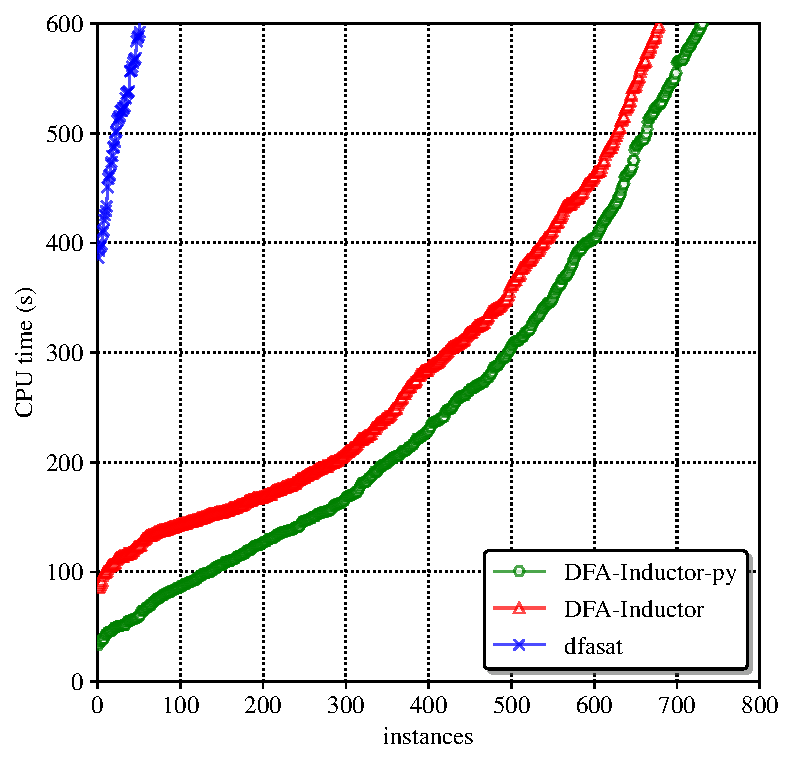
\includegraphics[width=\textwidth]{img/lata19/plots/cactus}
    \caption{Сравнение методов \texttt{DFA-Inductor}, \texttt{DFA-Inductor~2} и \texttt{DFASAT}, показывающее, число различных экземпляров задачи, решенное за определенное время}
    \label{img:plots:cactus}
  \end{subfigure}%
  \;\;
  \begin{subfigure}[b]{0.48\textwidth}
    \centering
    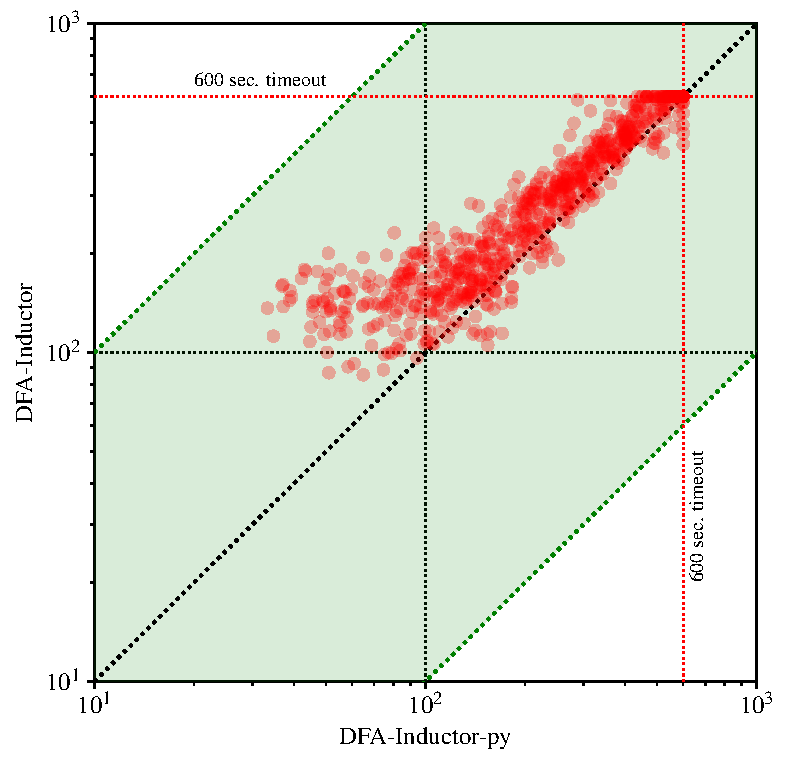
\includegraphics[width=\textwidth]{img/lata19/plots/scatter}
    \caption{Детальное сравнение методов \texttt{DFA-Inductor} и \texttt{DFA-Inductor~2}, сравнивающее их производительность в решении каждого экземпляра задачи}
    \label{img:plots:scatter}
  \end{subfigure}
  \caption{Результаты сравнения метода, использующего оригинальные BFS предикаты (\texttt{DFA-Inductor}), метода, использующего новые BFS предикаты (\texttt{DFA-Inductor~2}), и \texttt{DFASAT}}
  \label{img:plots}
\end{figure}


%----------------------------------------------------------------------------------------


\chresults{\ref{sec:space}}

